\footnotetext{Notes from Classical Mechanics by John R. Taylor, ch. 6}

\section{Two example problems}
The calculus of variations can be used to find a function $y(x)$ that minimizes a scalar quantity
that is expressed as an integral $\int_{x_0}^{x_1} f[y(x), y'(x), x] \dx$. Here are two such
problems:

\begin{question*}
  What is the shortest path between two points in a plane?
\end{question*}

\begin{proof}
  Let the points be $(x_0, y_0)$ and $(x_1, y_1)$ and let them be joined by some path $y(x)$ of
  length $S$. Consider a short section of the path of length $\Delta s$ above a section of the
  $x$-axis of length $\Delta x$, and make a linear approximation to the path in this region. The
  length of the hypotenuse is
  \begin{align*}
    \Delta s = \sqrt{(\Delta x)^2 + (y'(x)\Delta x)^2} = \sqrt{1 + y'(x)^2} \Delta x.
  \end{align*}

  Therefore a shortest path is a function $y(x)$ that minimizes
  \begin{align*}
    S = \int_{x_0}^{x_1} \d s = \int_{x_0}^{x_1} \sqrt{1 + y'(x)^2} \dx,
  \end{align*}
  \blue{
    \begin{align*}
      S[y](x_0, x_1) = \int_{x_0}^{x_1} \sqrt{1 + y'(x)^2}\d x.
    \end{align*}
  }

  with the constraint that the endpoints are fixed at $y(x_0) = y_0$ and $y(x_1) = y_1$.

  \todo{Find the function $y$ that minimizes this integral.}
\end{proof}


\begin{question*}
  In 1662 Fermat proposed that light, when passing from one point to another through a material with
  varying refractive index, takes the path which takes least time\footnote{\todo{In fact, the path
      taken is a stationary point with respect to the action? time? ...not necessarily least}}. What
  is this path?
\end{question*}

\begin{proof}
  Again consider a short section of the path of length $\Delta s$ above a section of the $x$-axis of
  length $\Delta x$. Let $c$ be the speed of light and $n$ be the refractive index in this
  region. This means that the light travels at speed $c/n$, and therefore takes time $(n/c)\Delta s$
  to pass along the hypotenuse. The refractive index $n$ can vary with both $x$ and $y$, therefore a
  least-time path is a function $y(x)$ that minimizes
  \begin{align*}
    T = \int_{x_0}^{x_1} n(x, y(x)) \d s = \int_{x_0}^{x_1} n(x, y(x)) \sqrt{1 + y'(x)^2} \dx,
  \end{align*}
  with the constraint that the endpoints are fixed at $y(x_0) = y_0$ and $y(x_1) = y_1$.

  \todo{Find the function $y$ that minimizes this integral.}
\end{proof}

A naive thought would be to somehow treat $y$ similarly to how a variable is treated when minimizing
a function in in basic calculus, i.e. differentiate the expression with respect to $y$. Recall that
the definition of derivative is
\begin{align*}
  f'(y_0) = \lim_{y_1 \to y_0}\frac{f(y_1) - f(y_0)}{||y_1 - y_0||}.
\end{align*}

\todo{I think this is nonsense and the reason is that multiplication (and therefore division) of
  functions is not defined (they can be treated as vectors, so can be added and scaled, but do not
  have an obviously appropriate multiplication operation). I don't think choosing a norm would
  necessarily be problematic.}

\section{The Euler-Lagrange equations}

\begin{proof}
  Note that in both example problems, the integral to be minimized can be viewed as a scalar-valued
  \emph{functional} $S$ that depends on the \emph{function} $y$:
  \begin{align*}
    S[y](x_0, x_1) = \int_{x_0}^{x_1} f[x, y(x), y'(x)] \dx.
  \end{align*}
  The arguments of the function $f$ that is integrated are \emph{not functions}! They are numeric
  values at a single point in the path: the current $x$ value, the current $y$ value, and current
  slope. We will attempt to stick to a notation wherein a symbol like $y$ is a function, and $y(x)$
  is a result of evaluating the function at input value $x$.

  We'll refer to $S$ as giving the \emph{cost} of traveling along the path $y$, from $(x_0, y_0)$ to
  $(x_1, y_1)$.

  Recall that we seek a least-cost path $y$, subject to the requirement that the endpoints are
  $y(x_0) = y_0$ and $y(x_1) = y_1$. Let $y$ be the least-cost path, and consider an alternative
  path $Y$ whose cost is greater than that of $y$. We can write $Y$ as
  \begin{align*}
    Y = y + \eta,
  \end{align*}
  where we are performing addition on domain-compatible
  functions\footnote{$(f + g)(x) := f(x) + g(x)$}. The difference function $\eta$ must satisfy
  $\eta(x_0) = \eta(x_1) = 0$ in order to restrict the space of functions to those with the same
  endpoints as $y$. Now introduce a parameter $\alpha \in \R$ and redefine $Y$ as\footnote{We are
    adding functions, and we are multiplying a function by a real scalar $\alpha$. The resulting
    function evaluates as $Y(x) = y(x) + \alpha\eta(x).$}
  \begin{align*}
    Y = y + \alpha\eta.
  \end{align*}

  So now we have a family of paths, parameterized by $\alpha$, all satisfying the endpoint
  requirement, and with the least-cost path corresponding to $\alpha=0$. We can reinterpret the cost
  $S$ so that it is a function of $\alpha$:
  \begin{align*}
    S[y](\alpha) &= \int_{x_0}^{x_1} f(x, Y(x), Y'(x)) \dx \\
                 &= \int_{x_0}^{x_1} f\(x, y(x) + \alpha\eta(x), y'(x) + \alpha\eta'(x)\) \dx.
  \end{align*}
  We are trying to find a path $y$ that is a minimum in the cost surface over the function space (or
  a maximum, or saddle point). For such a $y$ it must be the case that\footnote{In traditional
    notation, $\pdv{S}{\alpha}\Big|_{\alpha=0} = 0$.}
  \begin{align*}
    \del_\alpha S[y]\Big|_{\alpha=0} = 0.
  \end{align*}

  So, let's compute $\del_\alpha S[y]$ and use the fact that it must evaluate to zero at $\alpha=0$
  to obtain an equation that $y$ must obey. We'll assume that $f$ satisfies the (mild) conditions
  necessary to ``differentiate under the integral sign'', i.e. that
  \begin{align*}
    \del_\alpha S = \del_\alpha \int_{x_0}^{x_1} f(x, Y(x), Y'(x)) \dx
                 = \int_{x_0}^{x_1} (\del_\alpha f)(x, Y(x), Y'(x)) \dx.
  \end{align*}

  We have
  \begin{align*}
    Y  &= y + \alpha\eta \\
    Y' &= y' + \alpha\eta',
  \end{align*}
  and so from the chain rule we have
  \begin{align*}
    (\del_\alpha f)(x, Y(x), Y'(x)) &= (\del_{Y(x)} f)\del_\alpha
  \end{align*}

  \begin{align*}
    \pdv{f(Y, Y', x)}{\alpha} &= \pdv{f}{Y}\pdv{Y}{\alpha} + \pdv{f}{Y'}\pdv{Y'}{\alpha} \\
                              &= \pdv{f}{Y}\eta + \pdv{f}{Y'}\eta'.
  \end{align*}
  Plugging this into the expression for $\pdv*{S}{\alpha}$ and evaluating at $\alpha = 0$ we have
  \begin{align*}
    \int_{x_0}^{x_1} \(\eta\pdv{f}{y} + \eta'\pdv{f}{y'}\) \d x = 0.
  \end{align*}
  (I believe that $Y$ and $Y'$ have now become $y$ and $y'$ because we are evaluating at
  $\alpha=0$.)

  Now, recall integration by parts,
  $\int_a^b u \dv{v}{x} \d x = [uv]_a^b - \int_a^b v\dv{u}{x}\d x$, and apply it to the second term
  inside the integral:
  \begin{align*}
    \int_{x_0}^{x_1} \eta'\pdv{f}{y'} \d x = \Bigg[\eta\pdv{f}{y'}\Bigg]_{x_0}^{x_1} - \int_{x_0}^{x_1} \eta\(\dv{}{x}\pdv{f}{y'}\)\d x.
  \end{align*}
  Because $\eta$ was defined to be the difference between two candidate paths, as noted above we
  have that $\eta(x_0) = \eta(x_1) = 0$. Thus the first term (the ``endpoint term'' or ``boundary
  term'') is zero\footnote{According to Taylor this is common in physics, i.e. that the endpoint
    term is zero and thus integration by parts results in ``switching the prime'' from one factor to
    the other under the integral, and applying a negation.}. So now we have
  \begin{align*}
    \int_{x_0}^{x_1} \eta(x)\(\pdv{f}{y} - \dv{}{x}\pdv{f}{y'}\) \d x = 0.
  \end{align*}
  We now argue that this means that the difference-of-derivatives-function inside the integral is
  zero for all $x$. The reason is basically that this equality is true for \emph{any} $\eta(x)$. So
  suppose the difference-of-derivatives-function were not equal to zero for some $x$. Then we could
  construct an $\eta(x)$ that is non-zero for the same $x$ values that the
  difference-of-derivatives-function is non-zero for, the upshot being that we could construct
  things so that the value of the integral is non-zero; a contradiction. Therefore the
  difference-of-derivatives-function is zero for all $x$, and we have the Euler-Lagrange equations:
  \begin{align*}
    \pdv{f}{y} - \dv{}{x}\pdv{f}{y'} = 0.
  \end{align*}
  This is a system of differential equations which must be satisfied by any path that is stationary
  with respect to $f$.

  In SICM's functional notation, the Euler-Lagrange system of equations is
  \begin{align*}
    \del
  \end{align*}

\end{proof}
\section{SICM: Structure and Interpretation of Classical Mechanics}

\begin{definition*}~\\
  A \defn{derivative} of a function $f$ is the function $D f$. When $D f$ is evaluated at an input
  value the result is something which can be multiplied by an increment to the function's input to
  give a linear approximation to the increment in output:
  \begin{align*}
    f(x + \Delta x) \approx f(x) + (D f)(x)\Delta x.
  \end{align*}

  This definition holds for a function with $n$ inputs: the derivative function has $n$ inputs and
  $n$ outputs. Its output is something whose ``contraction''\footnote{I understand ``contraction''
    to refer to the multiplicative combination of one object with another object from the dual
    space. So for example, the matrix product of a row vector on the left with a column vector on
    the right.} with the increment in the function inputs gives a linear approximation to the
  increment in output.

  In the case where these inputs and outputs are $n$-dimensional vectors in $\R^n$ we can write this
  \begin{align*}
    f(\overrightarrow{x} + \overrightarrow{\Delta x}) \approx \overrightarrow{f(x)} + \overrightarrow{(D f)(x)} \cdot \overrightarrow{\Delta x}.
  \end{align*}
  Note that the value of the derivative $(D f)(x)$ is compatible for multiplication with the
  increment vector $\Delta x$. This is connected to the notions of column vector/row vector, linear
  functional\footnote{\url{https://en.wikipedia.org/wiki/Linear_form}}, vector/covector, tensor
  algebra etc. In SICM they refer to the output of the derivative function being a ``down tuple'',
  whereas all the other tuples here are ``up tuples''.

  A \defn{partial derivative} is one component of the derivative of a function of multiple inputs.

  So for a function $f:X \to Y$, the derivative is the function $D f:X \to X^*$, where $X^*$ is a
  space containing versions of $x \in X$ that are compatible for multiplication/contraction with
  $x$, i.e. a ``dual'' space.

  Suppose $f$ has an argument named $a$ that is of type $A$. Then the partial derivative of $f$ with
  respect to that argument is $\partial_a{f}:X \to A^*$.
\end{definition*}

\newpage
\subsection{The chain rule for a function with multiple inputs}

Suppose that a function $f$ measures something about a particle at a moment in time and depends on
three inputs:
\begin{enumerate}
\item the time $t$
\item the position $y(t)$
\item the velocity $y'(t)$.
\end{enumerate}
Further, suppose that the position and velocity in fact also depend on a parameter $\alpha$.

Now, let the value of $\alpha$ be changed slightly, to $\alpha + \Delta\alpha$, causing $y(t)$ to
change to $y(t) + \Delta y(t)$ and $y'(t)$ to change to $y'(t) + \Delta y'(t)$. These changes in
turn cause $f(t)$ to change to $f(t) + \Delta f(t)$.

The increment in $f(t)$ comes from two sources: the change in $y(t)$ and the change in $y'(t)$. We
can use the definition of partial derivative to make an approximation\footnote{The additive nature
  of this approximation needs to be justified I think.} to the increment in $f(t)$:
\begin{align*}
  \Delta f(t) \approx ~ &(\del_{y(t)} f)(t) \cdot \Delta y(t) \\
                    +   &(\del_{y'(t)} f)(t) \cdot \Delta y'(t).
\end{align*}
And we can do the same for $\Delta y(t)$ and $\Delta y'(t)$, replacing them with their linear
approximations given the increment in $\alpha$:
\begin{align*}
  \Delta f(t) \approx ~ &(\del_{y(t)} f)(t) \cdot (\del_\alpha y)(t) \cdot \Delta \alpha \\
                      + &(\del_{y'(t)} f)(t) \cdot (\del_\alpha y')(t) \cdot \Delta \alpha.
\end{align*}

The partial derivative $\del_\alpha f$ of $f$ with respect to $\alpha$ is defined to be a function
which, when evaluated at $t$, yields a quantity which multiplies $\Delta\alpha$ to give a linear
approximation to the increment $\Delta f(t)$:
\begin{align*}
  \Delta f(t) \approx \Delta\alpha \cdot (\del_\alpha f)(t).
\end{align*}
So we see that the quantity
\begin{align*}
    &(\del_{y(t)} f)(t) \cdot (\del_\alpha y)(t) \\
  + &(\del_{y'(t)} f)(t) \cdot (\del_\alpha y')(t)
\end{align*}
fits the definition of $(\del_\alpha f)(t)$.

This is normally written in a more streamlined fashion. In functional/operator notation it might be written
\begin{align*}
  \del_\alpha f = \del_y f \cdot \del_\alpha y + \del_{y'} f \cdot \del_\alpha y'.
\end{align*}
Alternatively, traditional (Leibniz) notation features a pattern of symbols that looks like
multiplication of fractions with cancellation:
\begin{align*}
  \pdv{f}{\alpha} = \pdv{f}{y} \pdv{y}{\alpha} + \pdv{f}{y'}\pdv{y'}{\alpha}.
\end{align*}
In both styles of notation we are multiplying and adding functions, with these operations defined
``pointwise'':
\begin{align*}
  (f + g)(x) &:= f(x) + g(x) \\
  (fg)(x)    &:= f(x)g(x).
\end{align*}







\subsection{Partial derivatives with respect to non-independent inputs}

Consider the function $f(x) = x^2 + 2x$. Clearly the derivative is $(D f)(x) = 2x + 2$.

However, suppose we choose to think of the function as $f(x, x^2) = x^2 + 2x$. In that case the
derivative is
\begin{align*}
  (D f)(x, x^2) = (x^2 + 2, 1).
\end{align*}




\section{The Euler-Lagrange equations: SICM functional notation}

Let $q:\R^+ \to \R$ be a function that maps time to coordinate in one-dimensional space.\footnote{In
  general, $q$ will map time to ``generalized coordinates'' of the system, i.e. whatever parameters
  are used to specify the state of the system at a moment in time}

Let $\eta$ be another function like $q$, with the same endpoints at the start and end time, and let
$\epsilon \in \R$, so that $q + \epsilon\eta$ is a different path with the same endpoints.

\blue{Note that the addition and scalar multiplication operators here are acting on a set of
  functions with the same range, and that they are defined as componentwise addition of the function
  values, and scalar multiplication of each function value:
  $(q + \epsilon\eta)(x) := q(x) + (\epsilon\eta)(x) := q(x) + \epsilon\eta(x)$. The set of path
  functions forms a vector space.}

Let $f[q]$ be a function that depends on a path $q$.

Define a \defn{variation of the function $f$ on the path $q$} to be
\begin{align*}
  \delta_{\eta}f[q] := \lim_{\epsilon \to 0} \frac{f[q + \epsilon\eta] - f[q]}{\epsilon}.
\end{align*}

\newpage
\footnote{Notes and exercises from Sussman et al. Structure and Interpretation of Classical Mechanics}
\subsubsection*{SICM ch. 1 Lagrangian Mechanics Exercise 1.4}
\begin{mdframed}
  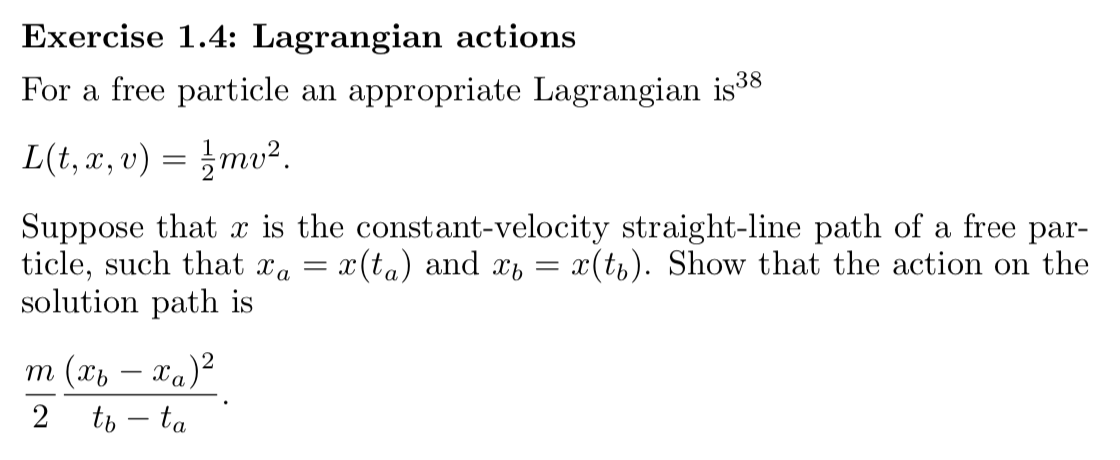
\includegraphics[width=400pt]{img/physics--classical-mechanics--sicm--1-4.png}
\end{mdframed}
The path function is
\begin{align*}
  x(t) = x_a + \frac{t - t_a}{t_b - t_a}(x_b - x_a).
\end{align*}
Therefore the velocity function is the constant function
\begin{align*}
  v(t) = (D x)(t) = \frac{x_b - x_a}{t_b - t_a}.
\end{align*}
Therefore the action is
\begin{align*}
  S[x](t_a, t_b) &= \int_{t_a}^{t_b}  \frac{1}{2}m \frac{(x_b - x_a)^2}{(t_b - t_a)^2} \d t \\
                 &= \frac{m}{2} \frac{(x_b - x_a)^2}{(t_b - t_a)^2}\int_{t_a}^{t_b} \d t \\
                 &= \frac{m}{2} \frac{(x_b - x_a)^2}{t_b - t_a}.
\end{align*}
